\chapter{Recherche}
\label{ch:Recherche}
In diesem Kapitel geht es um mehrere selbstdurchgeführte Befragungen zur Berechtigungsstruktur und der jährlichen Rezertifizierung.
Die jährliche Rezertifizierung ist die Überprüfung, ob die Mitarbeiter ihre Berechtigungen benötigen oder nicht.
Diese wird von den Teamleitern und Führungskräften durchgeführt, welche die Berechtigungsstruktur nutzen, um dies zu tun.
Dafür wurden drei verschiedene Gruppen befragt.
Die Ergebnisse sind die Grundlage für die Notwendigkeit einer sicheren und übersichtlichen Struktur sowie die Feststellung der Hauptprobleme der bestehenden Struktur.
Dabei wurde die Quelle \cite{HowSurvey} als primäres Grundgerüst verwendet, um die Befragung strukturiert und erfolgreich abzuschließen. Ebenso wurde die Quelle \cite{Survey} genutzt.

\section{Vorgehensweise}
\label{sec:Vorgehensweise}
Für die Befragung wurde zuerst analysiert, welche Stakeholder es gibt.
Bei der Analyse wurden die folgenden drei Stakeholder-Gruppen identifiziert:

\begin{itemize}
	\item \ac{FuT}
	\item IT-Systemspezialist
	\item Mitarbeiter
\end{itemize}
Die \ac{FuT} entsprechen den Stakeholdern, welche die Berechtigungsstruktur für die jährliche Rezertifizierung nutzen.
Diese haben eine hohe Priorität, da sie die Berechtigungsstruktur direkt verwenden und die Sicherheit der Struktur gewährleisten.
\newline
Die IT-Systemspezialisten sind die Stakeholder, die an der Berechtigungsstruktur gearbeitet haben.
Ebenso wie die Teamleiter und Führungskräfte haben die IT-Systemspezialisten auch eine hohe Priorität, weil sie die Struktur warten und verändern.
\newline
Die Mitarbeiter umfassen das restliche Arbeitspersonal.
Im Gegensatz zu den anderen beiden Stakeholdern haben die Mitarbeiter eine geringe Priorität, da diese weder die Struktur nutzen noch einen anderen Bezug zum Projekt haben.
\newline
\newline
Nachdem diese drei Stakeholder identifiziert worden sind, wurden spezifisch für diese drei Gruppen Fragenkataloge entwickelt.
Dabei ist das Ziel, festzustellen, welche die größten Probleme aus der Sicht der Teamleiter und Führungskräfte sowie IT-Systemspezialisten, sind.
Die Mitarbeiter wurden befragt, über wie viele Berechtigungen sie verfügen, die sie eigentlich nicht mehr benötigen.
Die große Herausforderung besteht dabei, die richtigen Fragen für die Fragenkataloge zu entwerfen.
Das Institut \ac{PRC} hat festgestellt, dass bei geschlossenen Fragen die Befragten zu einem großen Teil (über 90\%) eine der vorgeschlagenen Antworten gewählt haben. \cite{Survey}
Dies stellt ein Problem dar.
Wenn die Fragen geschlossen sind, dann kann es dazu führen, dass die Befragten nicht die Probleme angeben, die sie sehen.
Auf der anderen Seite sind offene Fragen auch eine Herausforderung, da es schwierig wird, die verschiedenen Antworten zu quantifizieren und auswerten zu können.
Ebenso ist die Wortwahl ein entscheidender Faktor.
In einer Studie von \ac{PRC} in 2003 wurden die Personen befragt, ob diese für oder gegen den Krieg in Irak sind, um Saddam Hussein's Herrschaft zu beenden.
68\% haben sich dafür und 25\% dagegen ausgesprochen.
Daraufhin wurde die Frage geändert zu, ob diese für oder den Krieg in Irak sind, um Saddam Hussein's Herrschaft zu beenden, selbst wenn es Tausende Verluste gibt.
Mit dieser Änderung haben nur noch 43\% dafür gestimmt und 48\% dagegen. \cite{Survey}
\newline
Dies ist relevant, da zum Beispiel bei der Befragung der Mitarbeiter bei einer falschen Formulierung der Gedanke kommen könnte, dass dieser mit der Beantwortung der Frage seine Zustimmung gibt, dass man ihm die genannten Berechtigungen entfernt.
Dies kann zu fehlerhaften Ergebnissen führen.
Deshalb müssen die Fragen gut überlegt sein.
\newline
\newline
Für die \ac{FuT} wurden die folgenden Fragen formuliert: 
\begin{itemize}
	\item Wie handhabbar ist für Sie der aktuelle Prozess der jährlichen Rezertifizierung der Vorgangsberechtigung ihrer Mitarbeiter?
	\item Was finden Sie am aktuellen Rezertifizierungsprozess gut?
	\item Was finden Sie am aktuellen Rezertifizierungsprozess schlecht?
	\item Was würden Sie gerne am aktuellen Rezertifizierungsprozess ändern?
	\item Was halten Sie von der Idee, dass Profile entweder nur noch (Unter-)Profile oder Profile ausschließlich Berechtigungen beinhalten?
	\item Soll es eine einheitliche Strukturierung für die Berechtigungsstruktur innerhalb der Bereiche geben?
	\item Haben Sie weitere Anmerkungen?
\end{itemize}
Die Fragen wurden größtenteils offen formuliert, um am besten die Probleme am bestehenden System zu identifizieren.
Dabei umfassen die ersten drei Fragen den Ist-Zustand der Berechtigungsstruktur und wie dieser durch die \ac{FuT} beantwortet werden.
Die Fragen vier, fünf und sechs fragen nach dem Soll-Zustand der Berechtigungsstruktur.
Dabei wurden auch konkrete Vorschläge in den Fragen unterbreitet, um einen ersten Eindruck von den \ac{FuT} zu erhalten.
Zum Schluss gab es noch die offene Frage, ob es weitere Anmerkungen gibt, um eventuelle Antworten und Anmerkung zu erhalten, die durch die vorherigen Fragen nicht abgedeckt wurden.
\newline
\newline
Für die IT-Systemspezialisten wurden die folgenden Fragen formuliert: 
\begin{itemize}
	\item Welche Erfahrung haben Sie mit der Berechtigungsstruktur entwickelt?
	\item Auf welche Probleme sind Sie im Zusammenhang mit der Berechtigungsstruktur gestoßen?
	\item Gibt es Sachen, die man bei der Berechtigungsstruktur beachten muss?
	\item Haben Sie Vorschläge, wie man die Berechtigungsstruktur besser gestalten könnte?
	\item Haben Sie weitere Anmerkungen?
\end{itemize}
Die erste Frage soll dazu anregen sich über das Thema Gedanken zu bilden, damit die folgenden Fragen einfacher zu beantworten sind.
Dabei soll die zweite Frage klarstellen, welche Herausforderungen die befragte Person mit der Struktur hatte.
Dies ermöglicht es, dann präventiv gegen diese vorzugehen und dies direkt mit in die neuen Konzepte zu integrieren.
Bei der dritten Frage sollen mögliche Ausnahmefälle genannt werden, die bei einem Konzept mitberücksichtigt werden müssten.
Anschließend wird gefragt, ob die Person eventuell sich selbst Gedanken gemacht hat, welche Möglichkeiten es gibt, um die aktuelle Struktur zu verbessern.
Zum Abschluss wird gefragt, ob es weitere Anmerkungen gibt, welche nicht von den vorherigen Fragen abgedeckt wurden.
\newline
\newline
Die Mitarbeiter haben die Frage bekommen:
\newline
\newline
\textit{Wie viele Vorgangsberechtigungen haben Sie in der Produktion von Hoblink, die Sie nicht mehr nutzen?}
\newline
\newline
Bei dieser Frage war es wichtig diese so zu formulieren, dass die befragte Person nicht den Eindruck bekommt, dass ich ihr die Berechtigungen wegnehmen möchte.
Dies würde ansonsten zu fehlerhaften Ergebnissen führen.
Dabei beschreibt Hoblink die Umgebungsoberfläche, die genutzt wird, um mit dem Host zu interagieren.
Die Befragung der Mitarbeiter dient dazu, um die Problematik der nicht optimalen Berechtigungsstruktur darzustellen und auch um feste Zahlen zu haben.
\newline
\newline
Dabei wurden die \ac{FuT} in der Informatikabteilung befragt, welche einen Kontakt mit der Berechtigungsstruktur haben.
Andere \ac{FuT} außerhalb der Informatik wurden nicht befragt, weil die Wahrscheinlichkeit zum zeitlichen Aufwand zu gering ist, hier nützliche Informationen zu erhalten.
Bei den IT-Systemspezialisten wurden alle Personen befragt, die mir bekannt waren.
Von den Mitarbeitern wurden zufällig von jedem Team von jeder Abteilung eine Person befragt.
Dies soll dazu dienen, dass man das Ergebnis skalieren kann.
\newpage
\section{Auswertung}
\label{sec:Auswertung}

Die folgenden Grafiken zeigen die Antworten der jeweiligen Befragungen.

\begin{figure}[h!]
 \centering
 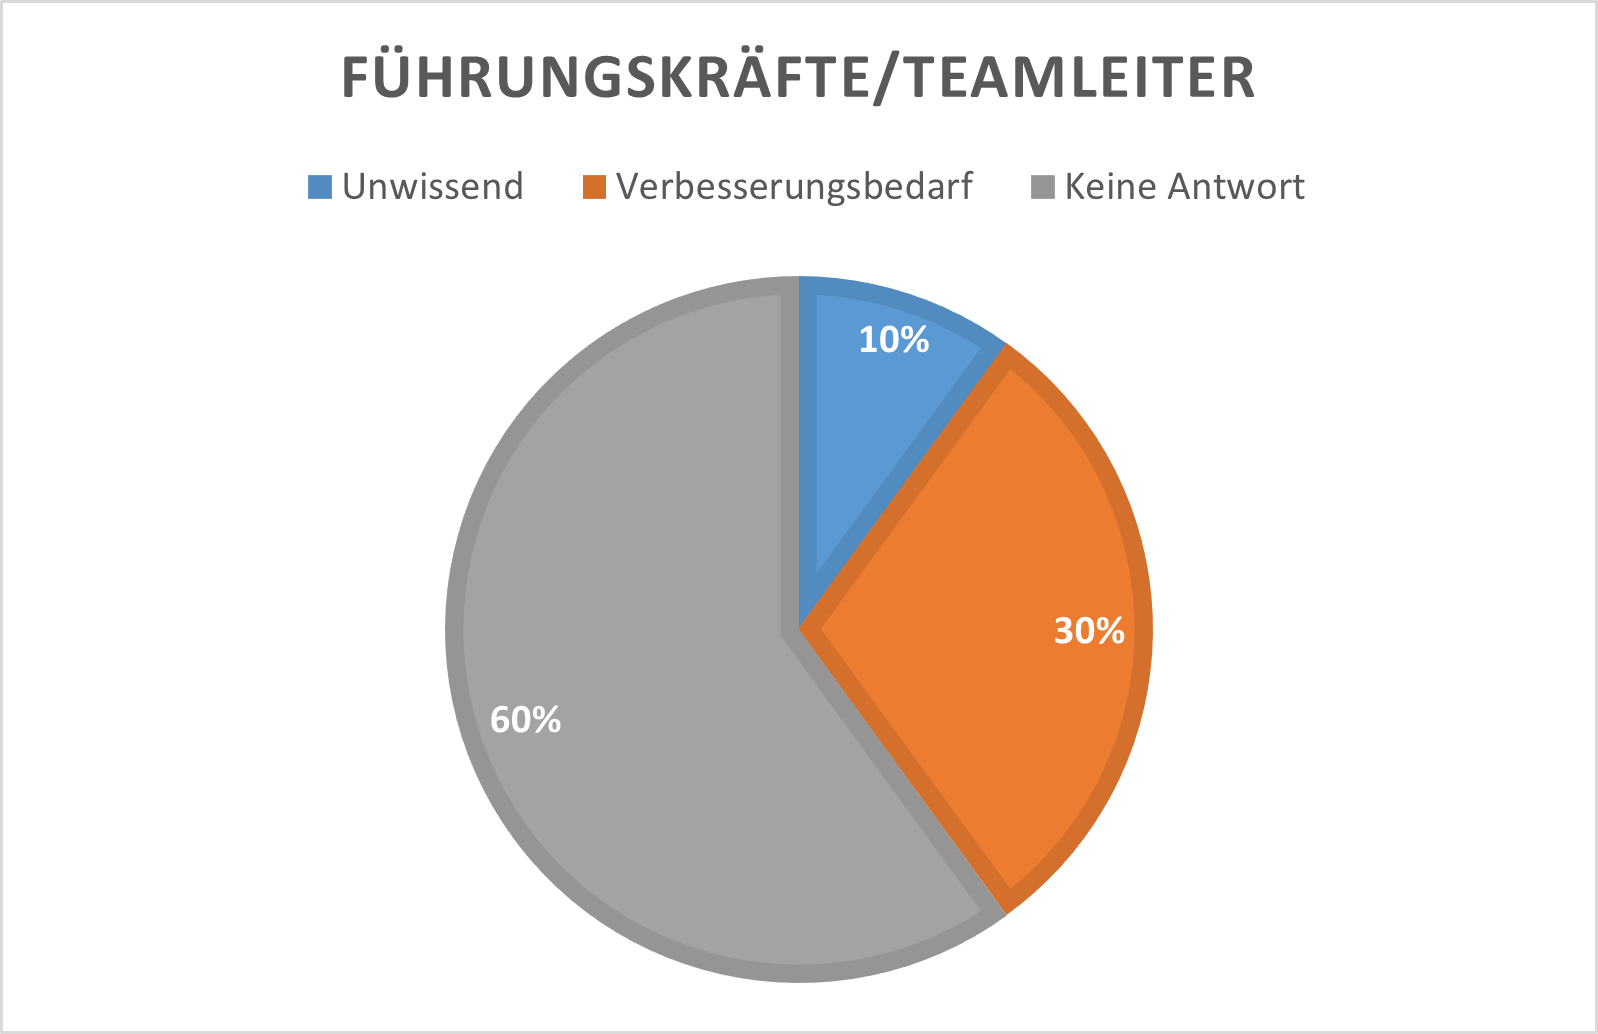
\includegraphics[width=1\textwidth]{gfx/Picture/FuT.PNG}
 \caption{Auswertung der Ergebnisse von den FuT}
 \label{fig:Fut}
\end{figure}
\begin{figure}[h!]
 \centering
 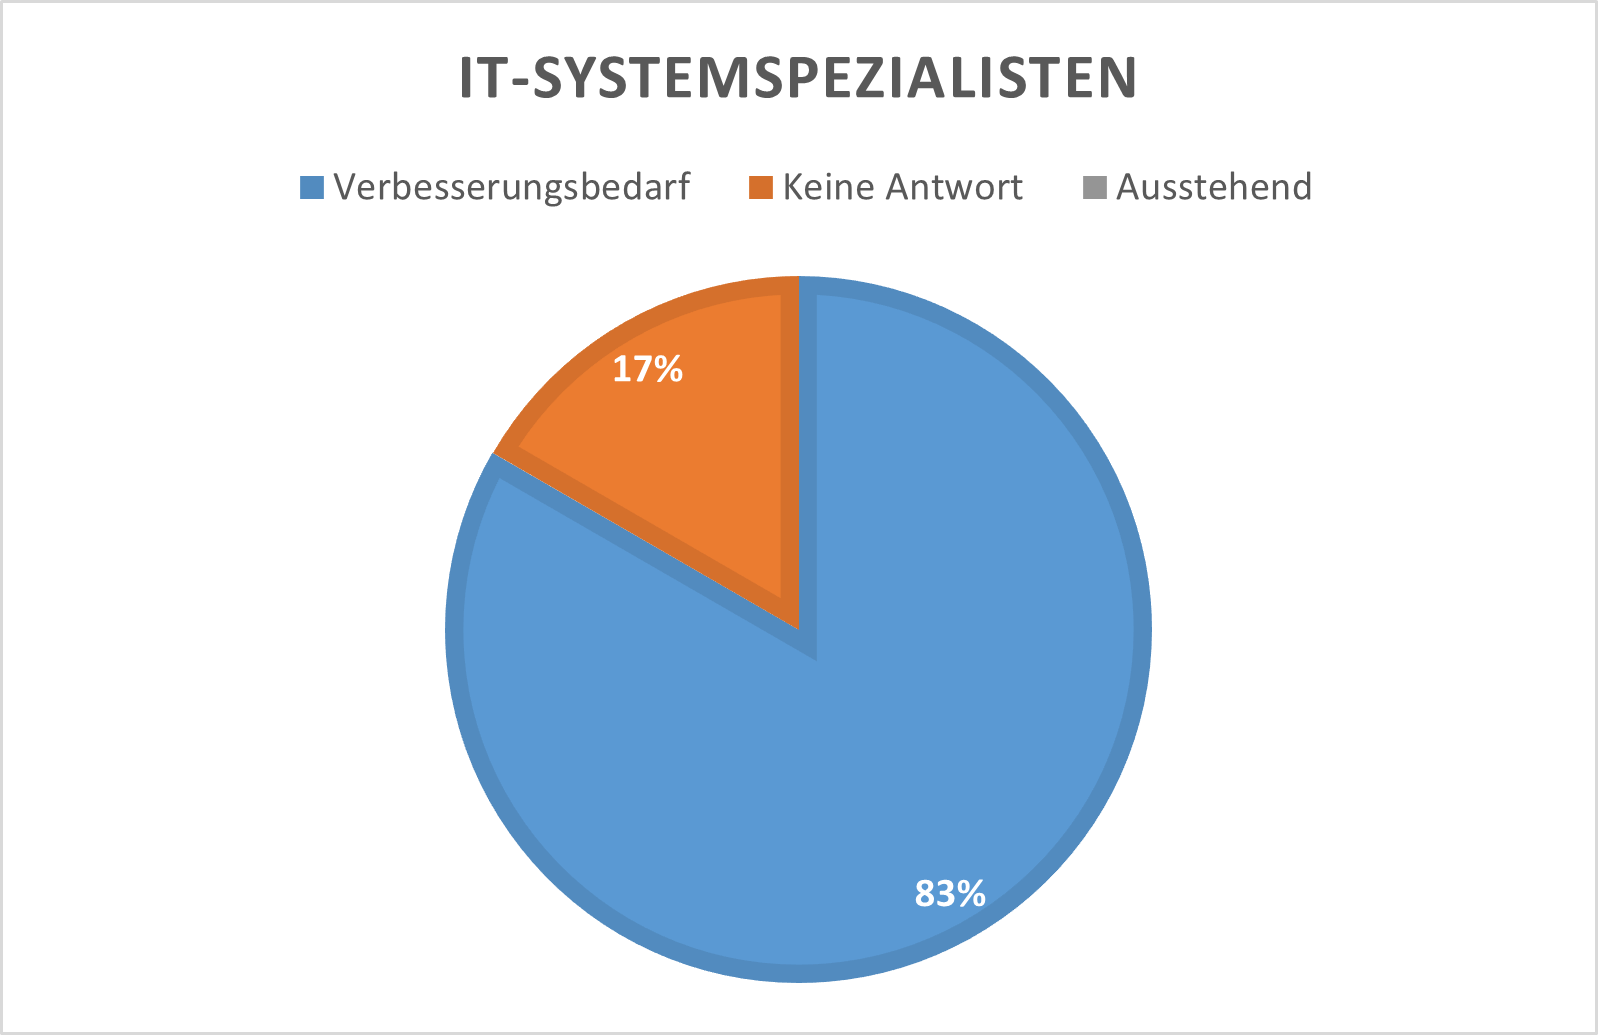
\includegraphics[width=1\textwidth]{gfx/Picture/IT.PNG}
 \caption{Auswertung der Ergebnisse von den IT-Systemspezialisten}
 \label{fig:IT}
\end{figure}
\begin{figure}[h!]
 \centering
 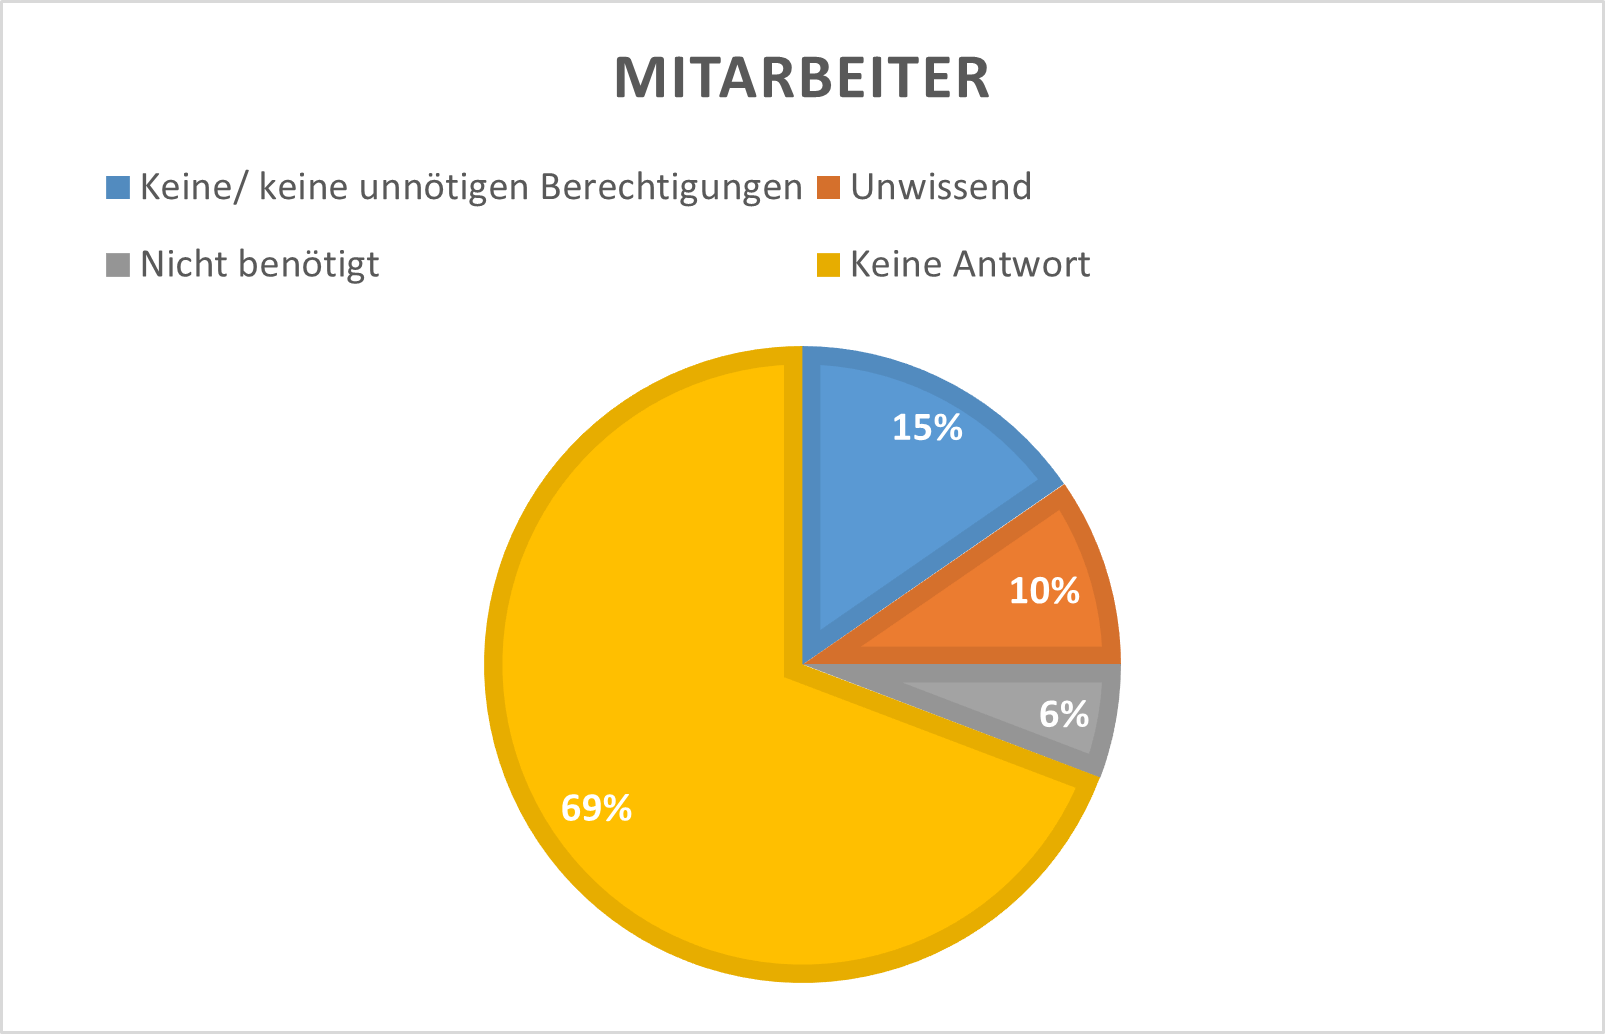
\includegraphics[width=1\textwidth]{gfx/Picture/Mitarbeiter.PNG}
 \caption{Auswertung der Ergebnisse von den Mitarbeitern}
 \label{fig:Mit}
\end{figure}
\newpage
Von den zehn befragten Teamleitern (Grafik \ref{fig:Fut}) haben vier an der Umfrage teilgenommen.
Von diesen vier haben drei angegeben, dass sie mit der aktuellen Struktur und Vorgehen umgehen können, es aber Verbesserungsbedarf besteht.
Dabei haben sie folgende Vorschläge gemacht:

\begin{itemize}
	\item Veraltete Vorgänge entfernen
	\item Helvetia Leben braucht keine HV/HI Mandanten
	\item Nur Änderung zum Vorjahr vergleichen
	\item Überprüfung von Sachgebieten an Stelle von Profilen/Vorgängen
\end{itemize}

Der erste Punkt wird aktuell sukzessive umgesetzt, ist jedoch nicht einfach und dauert lange.
Die Helvetia Versicherung ist aufgrund von gesetzlichen Regelungen in die Helvetia Leben und Helvetia Komposit aufgeteilt.
Dabei umfasst Helvetia Leben alle Versicherungen für die Person.
Dazu verfügt die Helvetia über drei Mandanten (HV, HI und HL).
Der HV-Mandant wird für den Zugriff von deutschen Daten verwendet.
HI im Gegensatz ist der Mandant für internationale Informationen.
Helvetia Leben hat explizit den HL-Mandanten.
Deswegen wurde vorgeschlagen, dass die Helvetia Leben Mitarbeiter die anderen beiden Mandanten nicht benötigen.
Jedoch ist dies nicht umsetzbar, da es Fälle gibt, bei denen diese auf die anderen Daten zugreifen müssen.
Zum Beispiel, wenn ein Vermittler nach Daten fragt, die nur über den HV-Mandanten verfügbar sind, muss der Mitarbeiter in der Lage sein, auf diese zuzugreifen.
\newline
Der Vorschlag, dass man nur die Änderungen zum Vorjahr vergleicht, würde den Aufwand massiv reduzieren, würde aber nicht mehr den Sinn der jährlichen Rezertifizierung erfüllen.
Das Problem besteht dabei, dass ein Mitarbeiter nach mehreren Jahren eine Berechtigung nicht mehr benötigt.
Wenn man dann nur den Vergleich zum Vorjahr betrachtet, würden dieser Person nie die älteren Berechtigungen entzogen werden können.
\newline
Die Überprüfung mittels Sachgebiete, anstelle von Profilen/Vorgängen, findet aktuell schon statt, da der Aufwand bei der Überprüfung der individuellen Profile/Vorgänge zu groß wäre.
Zudem bestände dann auch die große Wahrscheinlichkeit, dass versehentlich gewisse Profile/Vorgänge übersehen werden, welche eigentlich entfernt werden müssten.
\newline
\newline
Von den IT-Systemspezialisten haben sechs von sieben an der Befragung (\ref{fig:IT}) teilgenommen.
Im Interview mit den Befragten Personen haben diese verschiedene Anmerkung zum bestehenden System geäußert:

\begin{itemize}
	\item Chaotische Organisation
	\item Intransparent
	\item Schreckliches durcheinander
\end{itemize}

Wie man an den Bemerkungen erkennen kann, sehen die IT-Systemspezialisten das größte Problem bei der Hierarchie und dem Aufbau der Struktur.
Dabei haben sie verschiedene Vorschläge gemacht, wie man die Struktur aus ihrer Sicht verbessern kann.

\begin{itemize}
	\item Transparenter gestalten
	\item Baumstruktur "`verdammen"'
	\item Profile in Profilen abschaffen
	\item Eindeutige Struktur
	\item Konventionen
\end{itemize}
Auch wurde angesprochen, ob man das bestehende System nicht in RACF auslagern könnte.
Dabei wurde erwähnt, dass man sich darüber schon einmal Gedanken gemacht hatte.
Hierauf wird im Kapitel (\ref{sec:chapter05:racF}) näher eingegangen.
Zudem haben sie auch eine eigene Lösungsidee vorgeschlagen.
Diese wird in Kapitel (\ref{sec:chapter04:minimal}) erläutert.
\newline
\newline
Bei der Umfrage (\ref{fig:Mit}) von den Mitarbeitern haben 16 von 52 geantwortet.
Dabei haben sechs Personen angegeben, dass diese über gar keine oder keine unnötigen Berechtigungen verfügen.
Fünf haben geschrieben, dass sie nicht sicher sind, und weitere fünf haben angegeben, dass diese über Berechtigungen verfügen, die sie eigentlich nicht bräuchten.
Nach der Auswertung der Ergebnisse wurden die Ausssagen der Personen stichprobenartig mit deren Berechtigungen verglichen
Dabei wurde deutlich, dass zwei Personen, die angegeben hatten, dass diese über Berechtigungen verfügen und den Host nicht verwendeten, dennoch über Berechtigungen verfügen
Bei Nachfrage hatte sich herausgestellt, dass es sich um alte Accounts handelte, die sie für eine ehemalige Aufgabe benötigt hatten.
Diagramm \ref{fit:MitPruf} zegit die Auswertung der Ergebnisse unter Berücksichtigung dieses Sachverhaltes.
\begin{figure}[h!]
 \centering
 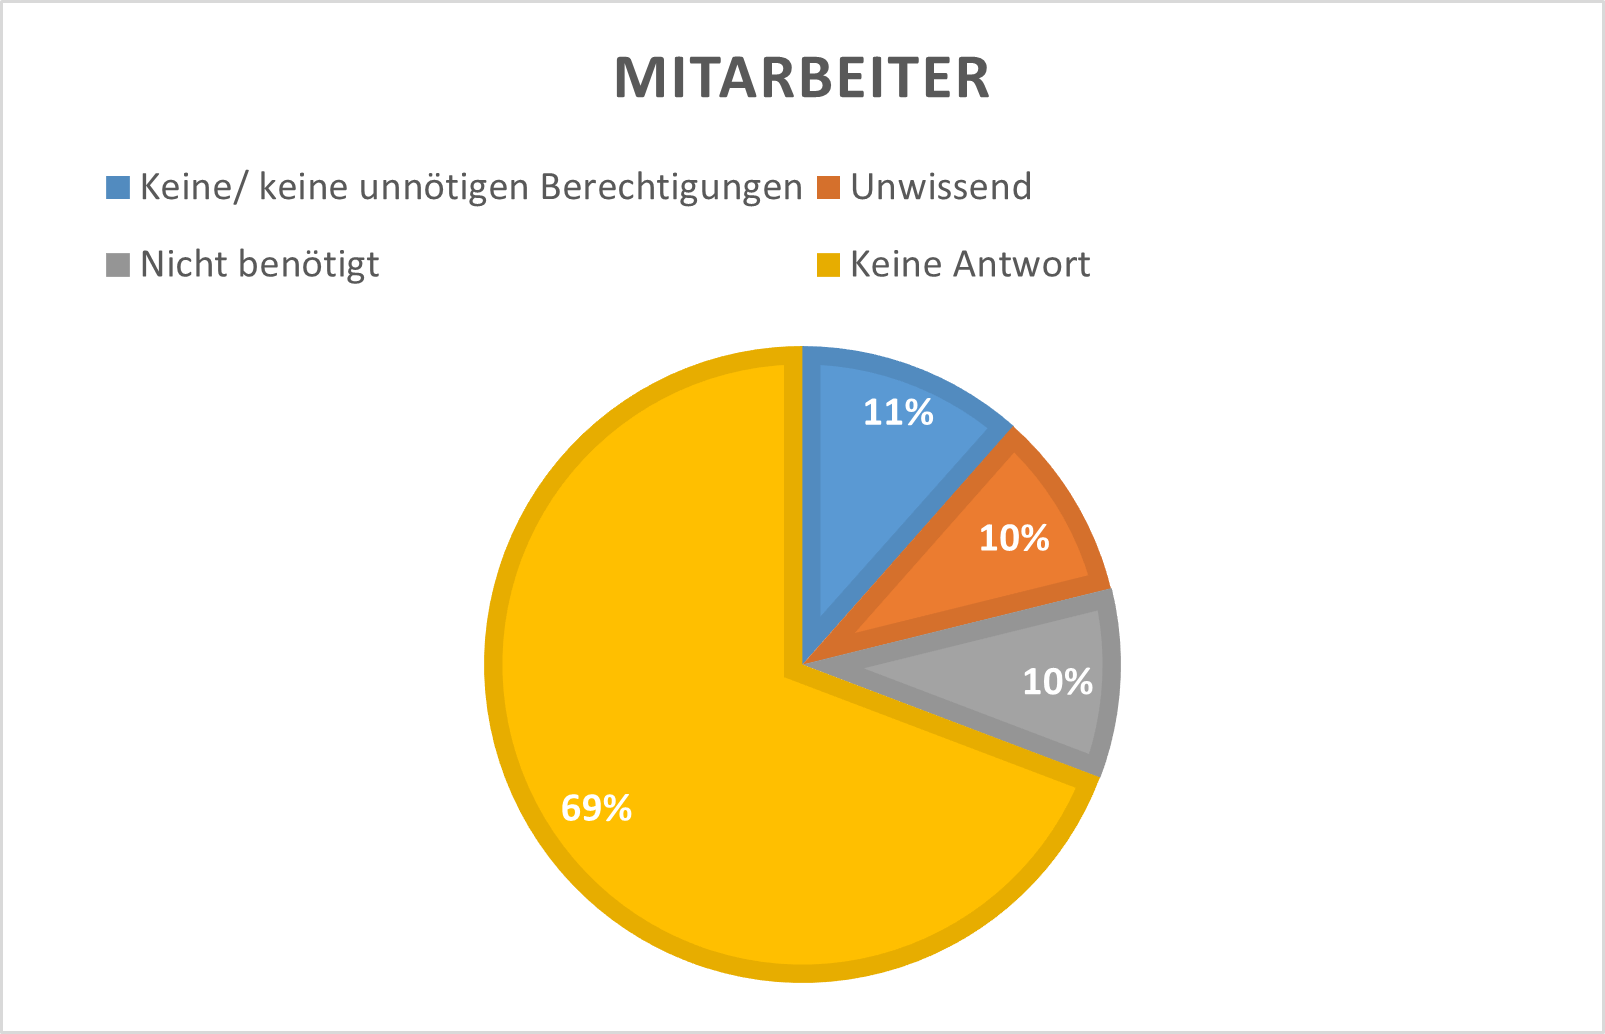
\includegraphics[width=1\textwidth]{gfx/Picture/Mitarbeiter(korregiert).PNG}
 \caption{Auswertung der Ergebnisse von den Mitarbeitern nach der Überprüfung}
 \label{fig:MitPruf}
\end{figure}
Wenn jetzt die Grafik betrachtet wird, kann erkannt werden, dass von den Personen, die geantwortet haben, 33\% zu viele Berechtigungen haben.
Es ist zu erkennen, dass nun ca, 33\% der Personen, die geantwortet haben, über zu viele Berechtigungen verfügen.
\section{Ergebnis}
\label{sec:Ergebnis}

Wie aus der letzten Grafik (\ref{fig:MitPruf}) erkennbar ist, besteht aktuell ein Problem.
Sollte einer dieser Mitarbeiter sein Passwort für diese Berechtigungen durch beispielsweise einen Phishingangriff weitergeben oder gegen das Unternehmen vorgehen wollen, könnte dies einen größeren, aber vermeidbaren Schaden anrichten.
Außerdem existiert eine mögliche Dunkelziffer bei der Befragung der Mitarbeiter, die nicht ehrlich geantwortet haben, weil diese eventuelle Angst haben, dass das Resultat der Befragung dafür sorgt, dass ihnen Berechtigungen entfernt werden.
Deswegen stelle ich die Annahme, dass 33\% der Mitarbeiter über Berechtigungen verfügen, die diese nicht benötigen.
Daher stellt die 33\% lediglich das Minimum dar.
Die Helvetia versendet jährlich Phishing-Mails, um die Mitarbeit zu trainieren, diese zu erkennen.
Dabei haben 10\% der Mitarbeiter ihre persönlichen Informationen preisgegeben (\ref{fig:Bef}).
Wäre dies kein Testfall, sondern ein echter Phishing-Angriff und einer der 33\% Mitarbeiter würde dem Angreifer diese Informationen geben, hätte der Angreifer es einfacher das gesamte System zu kompromittieren.
\newline
\newline
Genauso stellen deaktivierte Accounts ein Problem dar, da diese nicht mehr überprüft werden und bei der Reaktivierung keine Rezertifizierung stattfindet, ob diese Person noch sämtliche Berechtigungen benötigt.
Wodurch die Wahrscheinlichkeit besteht, dass diese zu viele Berechtigungen hat.
Zudem hat die Befragung der \ac{FuT} gezeigt, dass diese über kein tieferes Verständnis über die Struktur oder des Vorgehens verfügen, da diese Vorschläge unterbreitet haben, die entweder schon gemacht werden oder Vorgehensweisen, die problematisch sind.
Die Entwickler, die bisher an der Berechtigungsstruktur gearbeitet haben, haben verschiedene Ansätze und Probleme aufgezeigt, die im nächsten Kapitel ausführlicher behandelt werden.
\begin{figure}[h!]
 \centering
 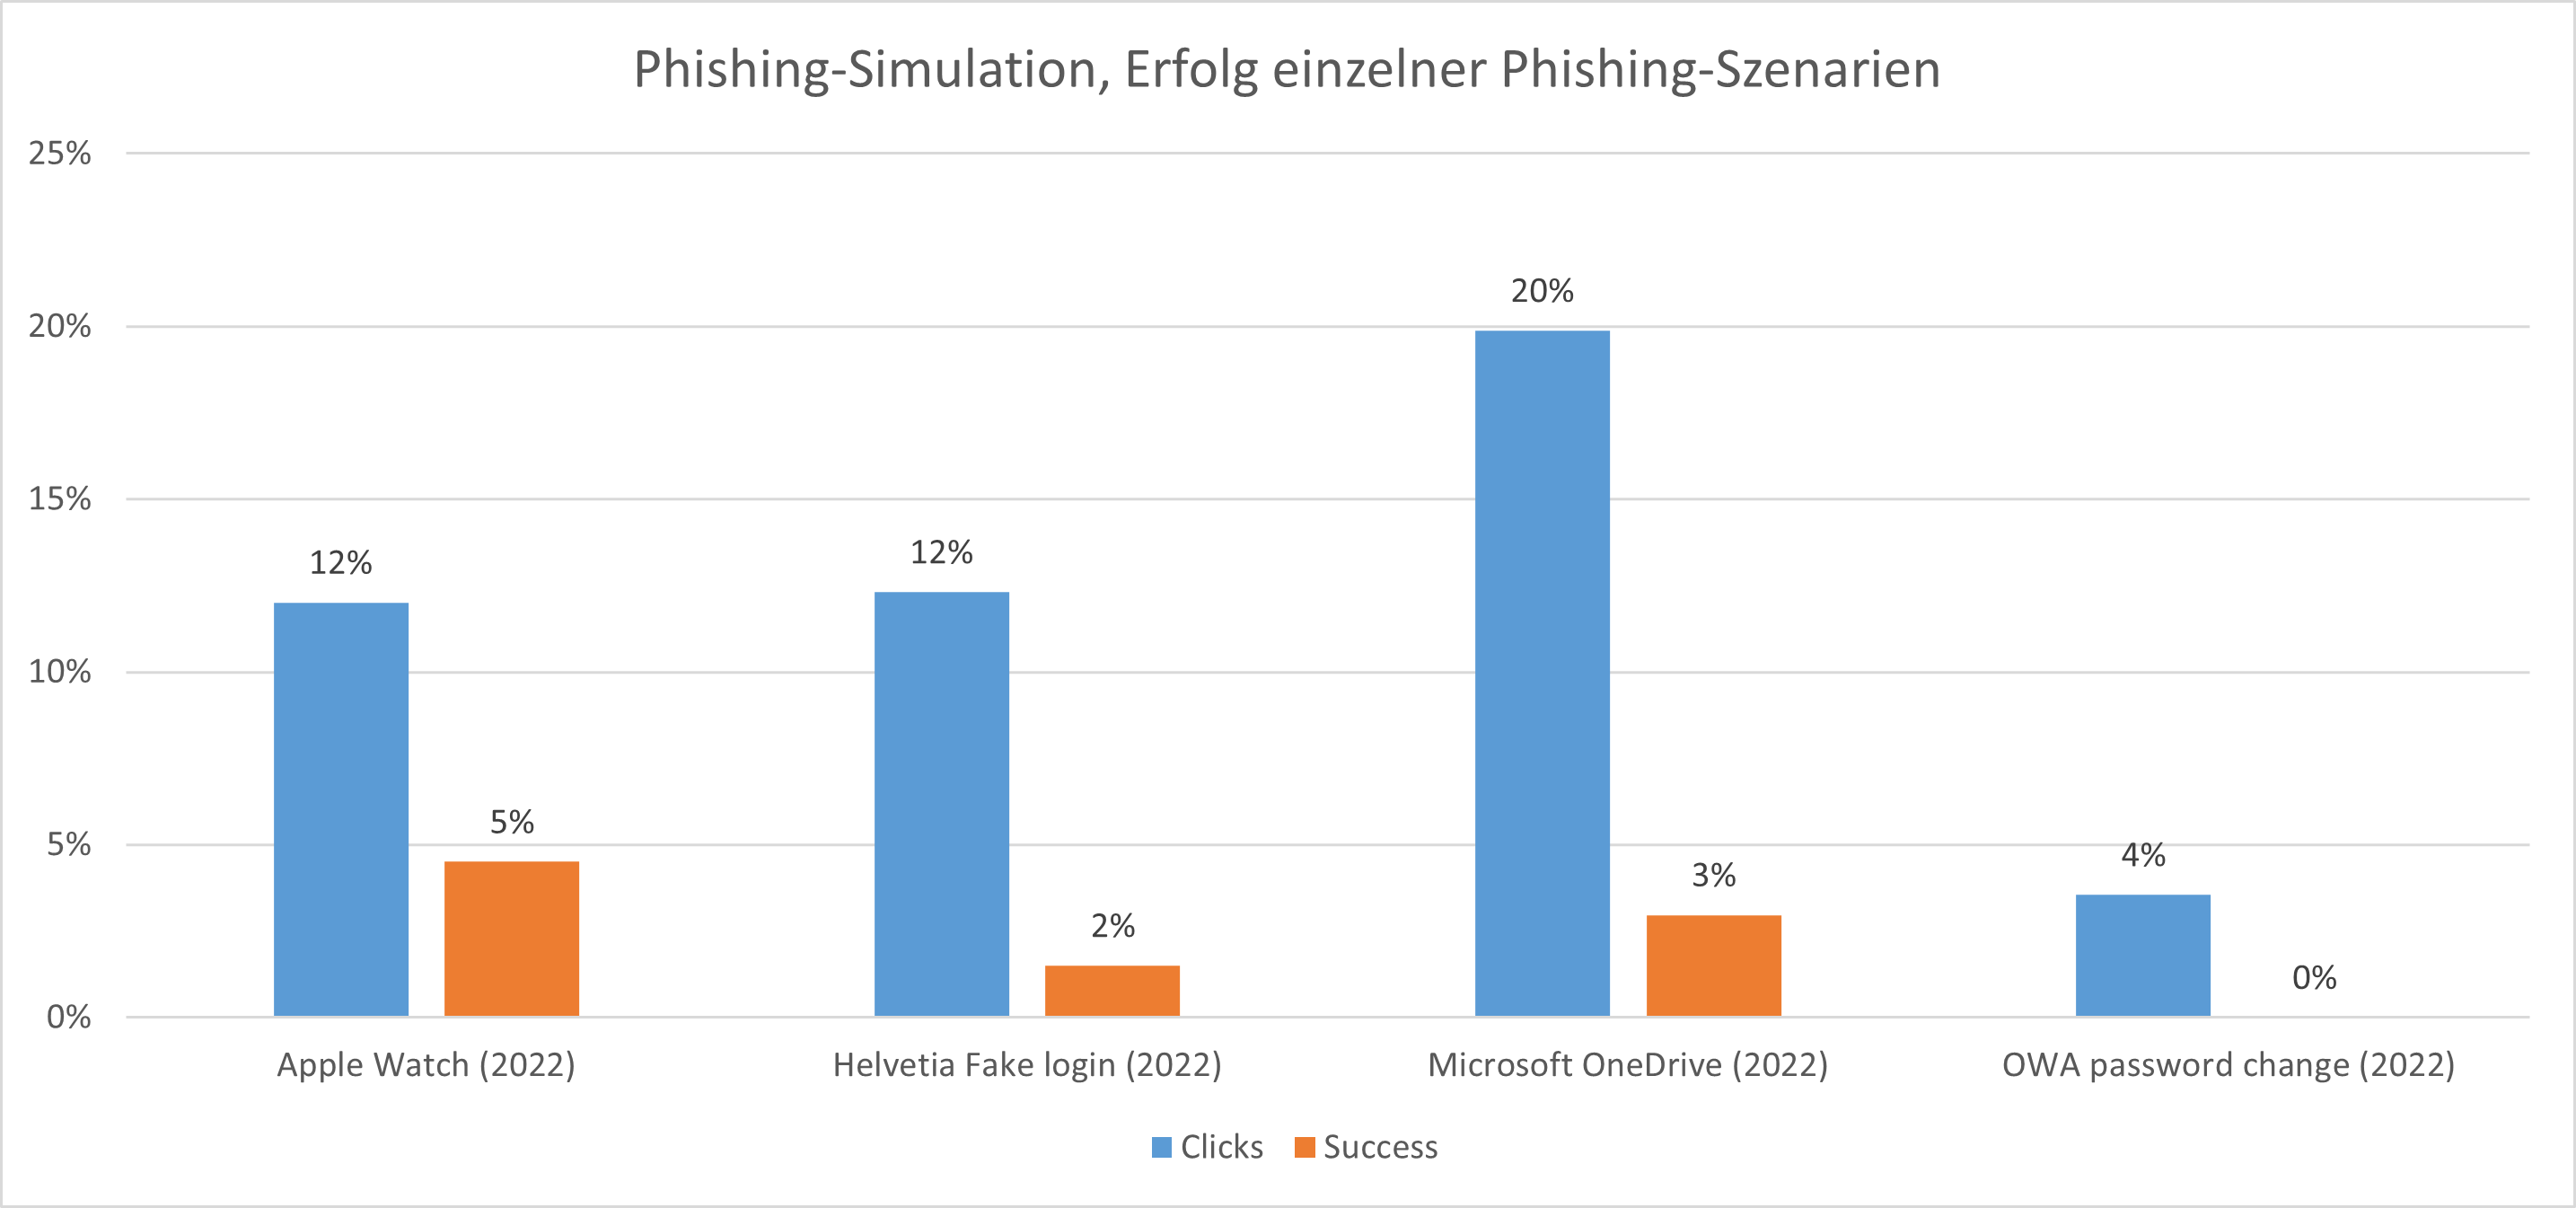
\includegraphics[width=1\textwidth]{gfx/Picture/Befragung.PNG}
 \caption{Phishing-Versuche von Helvetia an den eigenen Mitarbeitern \cite{Helvetia}}
 \label{fig:Bef}
\end{figure}

\section{Ist-Zustand}
\label{sec:chapter03:Ist-Zustand}
Der Ist-Zustand der Berechtigungsstruktur der Helvetia ist eine chaotische Organisation.
Zum Beispiel kann man im Bild \ref{fig:Teil} erkennen, dass das Profil PGE20 eine rekursive Beziehung hat.
Außerdem gibt es viele redundante Profile innerhalb eines Profils.
Das Profil Azub enthält zum Beispiel die Berechtigung PNE10, welche zwölfmal vergeben wird.
Dies macht es schwierig festzustellen, wer alles eine spezifische Berechtigung/Profil hat, da diese an verschiedenen Stellen vorkommt.
\newline
Zusätzlich gibt es Profile mit aufsteigenden Nummern wie zum Beispiel PNE10 und PNE20.
Dabei besteht das Problem, dass diese manchmal einen Bezug zueinander und manchmal gar keinen haben.
\begin{figure}[h!]
 \centering
 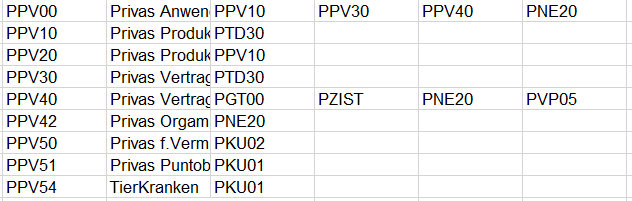
\includegraphics[width=1\textwidth]{gfx/Picture/Beispiel.PNG}
 \caption{Ausschnitt der Berechtigungsstruktur}
 \label{fig:Profile}
\end{figure}
Wie man in der Grafik \ref{fig:Profile} erkennen kann, hat das Profil PPV00 einen Bezug zu PPV10, PPV30 und PPV40, aber PPV54 hat gar keinen Bezug dazu.
Zudem sind dort Profile von anderen Fachbereichen vorhanden, welches das Risiko auf rekursive Beziehung erhöht und es schwierig macht, die Struktur zu verstehen.
In diesem Fall fehlt es an einer Richtlinie, welche vorgibt, wie die Beziehung zwischen diesen Profilen sein soll.
Diese sind notwendig, da es ansonsten für jemanden, welcher nicht über die notwendigen Fachkenntnisse verfügt, nicht in der Lage ist, die Berechtigungsstruktur zu verstehen.